\documentclass[11pt,a4paper]{article}
\usepackage[T1]{fontenc}
\usepackage[utf8]{inputenc}
\usepackage{lmodern}
\usepackage{amsmath}
\usepackage{amssymb}
\usepackage[margin=2.3cm]{geometry}
\usepackage{microtype}
\usepackage{booktabs}
\usepackage{tabularx}
\usepackage{graphicx}
\usepackage[font=small,labelfont=bf]{caption}
\usepackage{float}
\usepackage{enumitem}
\usepackage{xcolor}
\usepackage[colorlinks=true,linkcolor=blue!50!black,urlcolor=blue!50!black]{hyperref}

\setlist{nosep,leftmargin=*}
\setlength{\parskip}{0.5em}
\setlength{\parindent}{0pt}
\setlength{\emergencystretch}{3em}
\newcolumntype{Y}{>{\raggedright\arraybackslash}X}
\newcommand{\best}[1]{\textbf{#1}}

\title{\textbf{IRWA Final Project --- Part 3}\\[0.2em]\large Ranking and Filtering}
\author{\begin{tabular}{ccc}Èric Amargant & Josep Cardona & Jan Balayla\\\small u231867 -- NIA 284566 & \small u231747 -- NIA 284888 & \small u233694 -- NIA 286572\end{tabular}}
\date{November 2026}

\begin{document}
\maketitle

\textbf{GitHub repository:} \url{https://github.com/Janbacer/irwa-search-engine}\\
\textbf{Tag:} \texttt{IRWA-2026-part-3}\\
The \texttt{README.md} in the main folder explains how to install and run the code and how to choose the ranking
method. \texttt{project\_progress/part\_3/README.md} gives the details of this part.

In this part we rank the products returned by our conjunctive (AND) search in four different ways: TF-IDF with
cosine similarity, BM25, our own score, and word2vec with cosine similarity. All the code is in
\texttt{project\_progress/part\_3/}. The four methods are in \texttt{irwa\_ranking.py} (class \texttt{Ranker}), the
experiments are in \texttt{IRWA\_Part3.ipynb}, our labels are in \texttt{test\_queries\_labels\_all.csv}, and the
figures and result tables are in \texttt{figures/} and \texttt{results/}. We reuse the pre-processing of Part~1 and the
index, the AND search and the metrics of Part~2.

\textbf{Changes after the feedback on Part~2.} The test queries are now called \textbf{Q1--Q5} and the validation
queries \textbf{V1--V2}. Every table uses the same cut-offs ($K = 5, 10, 20$), and we show the results with figures.
The repository also has its final name, \texttt{irwa-search-engine} (the reports of Parts~1 and~2 still have the old
one).

%=====================================================================================================
\section{Set-up: search, queries and relevance labels}

We clean the query with the Part~1 function \texttt{preprocess\_text}, and the Part~2 AND search returns the products
that contain \emph{all} the query terms in \texttt{all\_terms}. The four methods rank \emph{the same} products, so only
the order changes. When two products have the same score, the one with the smaller \texttt{pid} goes first.

\begin{table}[H]
\centering\small
\caption{Queries, terms after pre-processing, AND matches and relevant products (Q1--Q5 were queries 3--7 in Part~2).}
\label{tab:queries}
\begin{tabularx}{\textwidth}{@{}l>{\raggedright}p{4.6cm}Yrr@{}}
\toprule
id & query & terms after pre-processing & matches & relevant\\
\midrule
Q1 & men white formal shirt slim fit & \texttt{men white formal shirt slim fit} & 25 & 9\\
Q2 & women floral print shirt & \texttt{women floral print shirt} & 35 & 27\\
Q3 & women black track pants with zip pockets & \texttt{women black track pant zip pocket} & 11 & 8\\
Q4 & women pure cotton t-shirt pack of 3 & \texttt{women pure cotton tshirt pack} & 140 & 26\\
Q5 & black running shoes for men & \texttt{black run shoe men} & 28 & 6\\
\midrule
V1 & women full sleeve sweatshirt cotton & \texttt{women full sleev sweatshirt cotton} & 566 & 13 of 20\\
V2 & men slim jeans blue & \texttt{men slim jean blue} & 225 & 10 of 20\\
\bottomrule
\end{tabularx}
\end{table}

\textbf{Relevance labels.} In Part~2 we only labelled the top~20 of TF-IDF for each test query (91 products). The new
methods put other products in their top~20, so this time we labelled \emph{every} AND match: 239 products, 148 of them
new (column \texttt{labelled\_in} of \texttt{test\_queries\_labels\_all.csv}). This way recall is exact and the four
methods are evaluated with the same labels. We used the same criteria as in Part~2:
\begin{itemize}
\item Q1: a formal, slim fit shirt for men, with white in its colours.
\item Q2: a women's shirt with a floral print (unstitched shirt \emph{fabric} is not a shirt).
\item Q3: black track pants for women (not for men, and not trousers).
\item Q4: a women's t-shirt sold in a \emph{pack of 3}.
\item Q5: black running shoes for men (not for women, and not other kinds of shoe).
\end{itemize}

\textbf{Evaluation.} We use the Part~2 metrics (\texttt{irwa\_evaluation.py}): P@K, R@K, AP@K (its mean is MAP), F1@K,
RR (its mean is MRR) and NDCG@K, with $K = 5, 10, 20$. V1 and V2 only have 20 labelled products each (and only 8 of the
20 of V2 contain all the query terms), so their results depend on very few products.

%=====================================================================================================
\section{Ranking with TF-IDF, BM25 and our score (point 1)}

\subsection{TF-IDF + cosine similarity}
\[
w(t,d) = tf(t,d)\cdot \log\frac{N}{df_t}, \qquad
\text{score}(q,d) = \cos(q,d) = \frac{\sum_{t\in q} w(t,q)\,w(t,d)}{|q|\;|d|}
\]
Here $tf(t,d)$ is the number of times the term $t$ appears in the product, $df_t$ is the number of products that
contain it, and $N = 28{,}080$. $|d|$ is the length of the TF-IDF vector of the whole product (all its terms, not only
the query terms), so the score is a real cosine. We use the raw count as $tf$. The $tf$ of the labs (the count divided
by the length of the vector of counts) gives exactly the same cosine: this division is the same for all the terms of a
product, and the cosine already divides by the length of the vector. In Part~2 the score was not a real cosine,
because we divided the counts by their length but then multiplied them by the idf, so the final vector did not have
length~1. In Part~3 we fixed this.

\subsection{BM25}
\[
\text{BM25}(q,d) = \sum_{t\in q} \log\frac{N}{df_t}\cdot \frac{tf(t,d)\,(k_1+1)}{tf(t,d) + k_1\left(1 - b + b\,\frac{|d|}{avgdl}\right)}
\]
The idf is the same as in TF-IDF. Here $|d|$ is the number of terms of the product, $avgdl = 43.9$ is the average, and we
use the usual values $k_1 = 1.2$ and $b = 0.75$. Figure~\ref{fig:sat}b shows the mean NDCG@10 for other values. Some
length normalisation is needed ($b = 0$ gives the worst results, 0.47--0.49), and a smaller $b$ would be better for our
short products (0.68 with $k_1 = 0.5$ and $b = 0.25$, against 0.61). We still keep the standard values, because choosing the
best cell would over-fit our five queries: the values would work well on them, but not necessarily on other queries.

\subsection{How TF-IDF and BM25 differ}
\label{sec:diff}
Both scores give more weight to rare query terms (idf) and prefer short products, but they do it in different ways:

\begin{table}[H]
\centering\small
\caption{TF-IDF + cosine compared with BM25.}
\label{tab:tfidf-bm25}
\begin{tabularx}{\textwidth}{@{}lYY@{}}
\toprule
 & TF-IDF + cosine & BM25\\
\midrule
repeated terms & linear: every repetition counts the same, so 10 occurrences weigh 10 times one & saturates: the
extra repetitions count less and less, at most $k_1 + 1 = 2.2$ times one (Figure~\ref{fig:sat}a)\\
length & divides by the length of the whole TF-IDF vector, which grows with the number of terms \emph{and} with how rare
they are & divides by the number of terms compared with the average, softened by $b$\\
query & a TF-IDF vector, so a repeated query word counts more & each different query term counts once\\
parameters & none & $k_1$ and $b$\\
\bottomrule
\end{tabularx}
\end{table}

\begin{figure}[H]
\centering
\begin{minipage}{0.49\textwidth}\centering
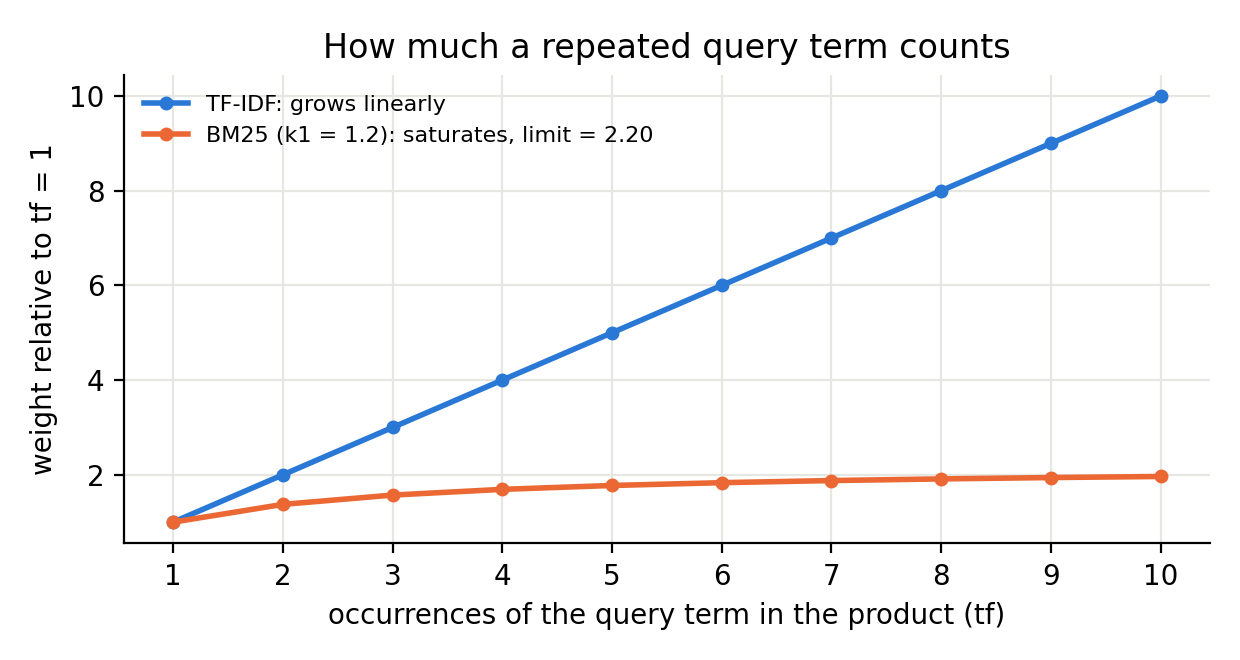
\includegraphics[width=\textwidth]{figures/tf_saturation.png}\\\small (a)
\end{minipage}\hfill
\begin{minipage}{0.46\textwidth}\centering
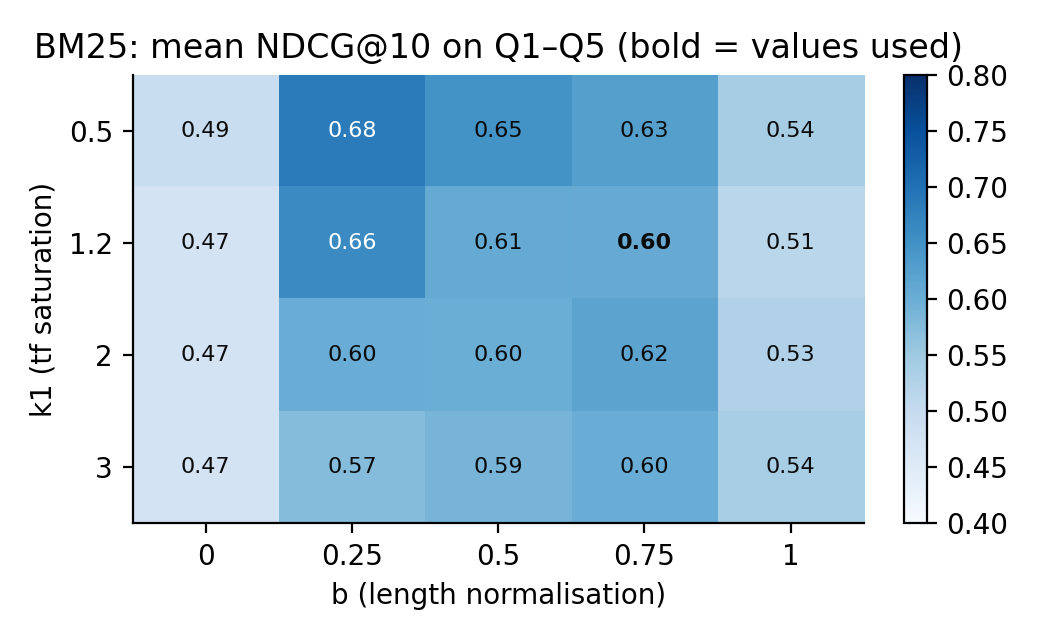
\includegraphics[width=\textwidth]{figures/bm25_parameters.png}\\\small (b)
\end{minipage}
\caption{(a) Weight of a query term depending on how many times it appears, compared with one occurrence (for a product
of average length). (b) BM25: mean NDCG@10 on Q1--Q5 for different $k_1$ and $b$ (in bold, the values we use).}
\label{fig:sat}
\end{figure}

\begin{figure}[H]
\centering
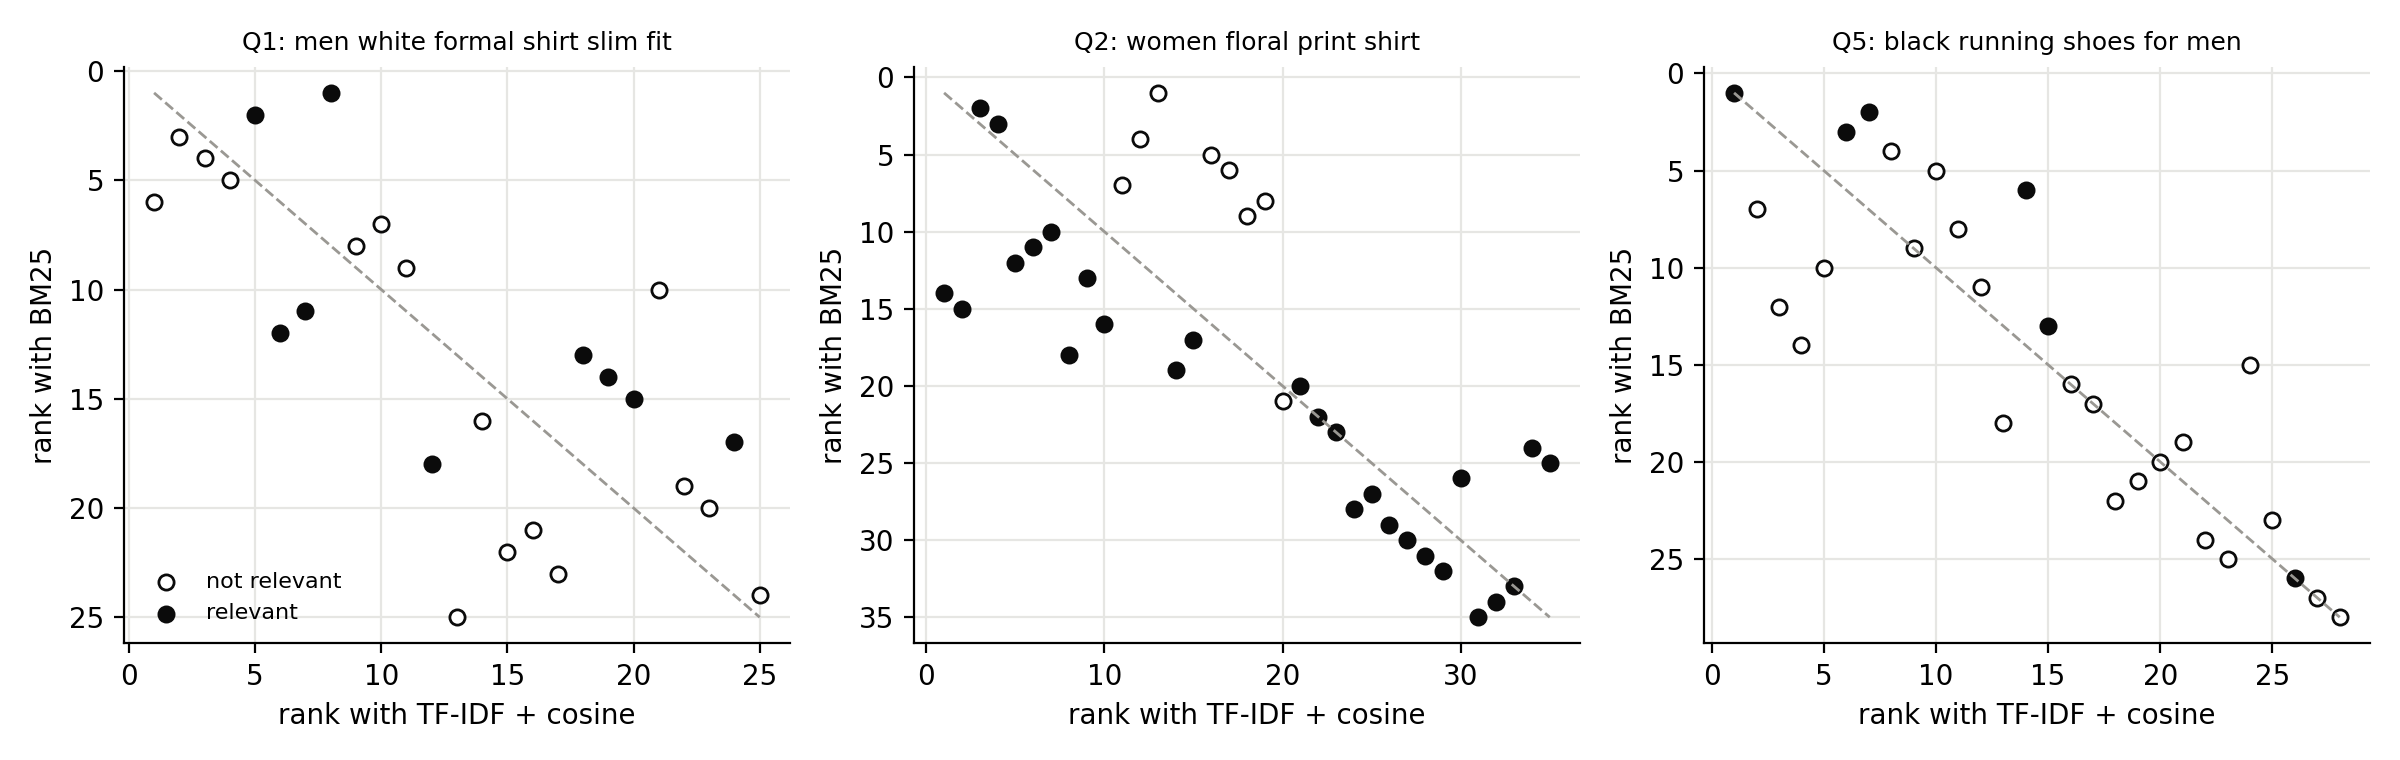
\includegraphics[width=\textwidth]{figures/tfidf_vs_bm25_ranks.png}
\caption{Each point is one AND match: $x$ is its position with TF-IDF + cosine and $y$ its position with BM25 (position~1
at the top left). Filled points are relevant products. A point on the diagonal has the same position in both
rankings; a point above it is ranked higher by BM25, and a point below it is ranked higher by TF-IDF. The points far
from the diagonal are the products on which the two scores disagree.}
\label{fig:ranks}
\end{figure}

Figure~\ref{fig:ranks} shows in which products the two rankings disagree. Two examples explain the differences:
\begin{itemize}
\item \textbf{Q1 (repeated terms).} The empty points at $x = 1$--$4$ are casual shirts: TF-IDF puts them first, but
BM25 moves them down. The first one is short (25 terms, TF-IDF norm 12.1) and contains the common word \texttt{shirt}
four times, but \texttt{formal} and \texttt{white} only once. TF-IDF counts the four \texttt{shirt}s fully, so this
product gets a high score. BM25 saturates the repetitions, so the extra \texttt{shirt}s count much less, and it puts
first a formal shirt that contains \texttt{formal} and \texttt{white} twice each, even if this shirt is longer (33
terms, norm 21.0). This is the filled point at $x = 8$, $y = 1$: it was 8th with TF-IDF and is 1st with BM25.
\item \textbf{Q2 (length normalisation).} The group of empty points at the top ($y = 1$--$9$, $x = 11$--$19$) are
shirt fabrics: BM25 puts 7 of them in its top~9 (NDCG@10 0.31), while TF-IDF puts all of them after position 10
(NDCG@10 1.00). The best fabric and the best women's shirt contain the query terms the same number of times and have
the same length (20 terms). BM25 only looks at these two things, so it gives both the same score, and the fabric comes first only
because of its \texttt{pid}. TF-IDF also looks at
the other words: the fabric contains rare words like \texttt{rayon} and \texttt{unstitch}, which make its TF-IDF vector
longer (19.4 against 14.0), so its cosine is lower.
\end{itemize}

\begin{table}[H]
\centering\small
\caption{Pros and cons of TF-IDF + cosine and BM25.}
\begin{tabularx}{\textwidth}{@{}lYY@{}}
\toprule
 & pros & cons\\
\midrule
TF-IDF + cosine & simple and without parameters; queries and products are vectors of the same kind (we could also
compare two products); products full of unrelated rare words go down (Q2) & a repeated word keeps adding score; we
cannot adjust the length normalisation; it prefers short products that contain each query word once (the casual shirts
of Q1, the wrong pack sizes of Q4)\\
BM25 & it rewards containing \emph{more different} query terms over repeating one; the length normalisation can be
adjusted; better MRR than TF-IDF (0.90 against 0.68) & two parameters
that depend on the collection; it treats the product as one bag of words, so a word in the title counts the same as
one in the description; it can favour short products too much (the fabrics of Q2), so it has a lower P@10 (0.46
against 0.58)\\
\bottomrule
\end{tabularx}
\end{table}

BM25 is better on Q1, Q4 and Q5, TF-IDF on Q2, and both do the same on Q3 (Figure~\ref{fig:perquery}). Both fail for the
same reason: they count words, but they do not know \emph{where} in the product each word appears. Our score is built to
solve this.

\subsection{\texorpdfstring{Our score: BM25F $\times$ title factor $\times$ quality}{Our score: BM25F x title factor x quality}}
\label{sec:ours}
\[
\text{ours}(q,d) = \underbrace{\text{BM25F}(q,d)}_{\text{text, by field}} \times
\underbrace{\Bigl(1 + w_{title}\,\frac{|q \cap \text{title}(d)|}{|q|}\Bigr)}_{\text{title factor}} \times
\underbrace{\Bigl(1 + 0.1\,\frac{\text{rating} - 1}{4} + 0.05\,\frac{\text{discount}}{100}\Bigr)\, s_{stock}}_{\text{quality factor}}
\]
The errors above come from query words that appear in the wrong field: ``formal'' in the details of a casual shirt
(Q1), ``men'' only in the sub-category ``Men's Footwear'' of women's shoes (Q5), and ``shirt'' in the title of a fabric
(Q2). Our score has three parts:

\begin{itemize}
\item \textbf{BM25F} (BM25 with field weights). In Part~1 we saw that the query terms of the relevant products are in the
title and in the product details, while the description has as many query terms for the non-relevant products. So each
field has a weight (title~3, details~2, brand~1, sub-category~0.5, description~0.5) and its own length normalisation,
and we add the weighted counts \emph{before} the saturation:
$\widetilde{tf}(t,d) = \sum_{f} w_f\,\frac{tf_f(t,d)}{1 - b + b\,|d_f| / avg|d_f|}$ and
$\text{BM25F}(q,d) = \sum_{t\in q} \log\frac{N}{df_t}\,\frac{\widetilde{tf}\,(k_1+1)}{\widetilde{tf} + k_1}$.
\item \textbf{Title factor} ($w_{title} = 1$). The score is multiplied by up to 2 when all the query terms are in the
title. The title says what the product \emph{is}, and gender words have a low idf, so the field weights alone are not
enough.
\item \textbf{Quality factor} (numeric fields). The rating adds up to $+10\%$, the discount up to $+5\%$, and the 1,644
out-of-stock products are multiplied by $s_{stock} = 0.5$ (they still match the query, so we keep them, but lower). A
missing rating (2,261 products) gets the mean rating, so it does not help or hurt, and a missing discount (855) counts
as 0. For products in stock the factor goes from 1.000 to 1.141, so it only reorders products with similar text scores
(87\% of the titles are repeated) and it can never put a bad text match above a good one. We keep the weights small
because the rating does not come with a number of reviews and the discount is decided by the seller.
\end{itemize}

\begin{table}[H]
\centering\small
\caption{Ablation of our score: we add the parts one by one (mean over Q1--Q5).}
\label{tab:ablation}
\begin{tabular}{@{}lccc@{}}
\toprule
variant & P@10 & MAP@10 & NDCG@10\\
\midrule
BM25 & 0.460 & 0.793 & 0.605\\
BM25F & 0.580 & 0.788 & 0.729\\
BM25F $\times$ title factor & \best{0.740} & 0.903 & 0.885\\
BM25F $\times$ title $\times$ quality (\textbf{our score}) & \best{0.740} & \best{0.915} & \best{0.890}\\
\bottomrule
\end{tabular}
\end{table}

Most of the improvement comes from the field weights and the title factor (NDCG@10 goes from 0.61 to 0.73 and then to
0.89). The title factor is not tuned to our queries: with $w_{title} = 0.5$, 1 or 2 we get 0.889, 0.890 and 0.890, so
the result does not depend on its exact value. The quality
factor changes little in the metrics (our labels do not look at stock, rating or price), but it breaks the ties between
equivalent products. With our score, 8 of the first 10 results of Q1 are relevant, the top~5 of Q2 and Q5 are all
relevant, and the fabrics and the women's shoes go down.

\textbf{Pros:} it uses the structure of the product (a word in the title counts more than one in the description),
which gave the biggest improvement of all our experiments; it uses information that the text does not have (stock,
rating, discount); it is easy to explain and to change (all the weights are constants in \texttt{irwa\_ranking.py});
and missing values do not change the score. \textbf{Cons:} it has more parameters. We set them from Part~1 and did not
tune them, but we chose them knowing how these same queries failed in Part~2, so the test results may be a bit
optimistic. The quality factor follows criteria that our labels do not include (it lowers V1, see
Section~\ref{sec:compare}), the rating and the discount are weak signals, and nothing in the score can see the pack size
of Q4.

%=====================================================================================================
\section{word2vec + cosine similarity (point 2)}

We train word2vec (\texttt{gensim}) on \emph{our own corpus}, because a pre-trained model (for example Google News) would
not know \texttt{tshirt} or stems like \texttt{sleev}. Each title, product details and description is one sentence of
Part~1 terms (73,037 sentences). We use skip-gram (it is better for rare words), 100 dimensions, a window of 5, the
words seen at least twice (4,540 words) and 10 epochs. With one worker and a fixed seed we get the same vectors on every
run (training takes about 30~seconds). A product is the \emph{average} of the vectors of its \texttt{all\_terms}, a
query is the average of the vectors of its terms, and the score is the cosine between them. The top-20 lists of Q1--Q5
are in Appendix~\ref{app:w2v} and in \texttt{results/word2vec\_top20.csv}.

word2vec is perfect on Q2 (NDCG@10 = 1.00), but it is the worst method on Q1 (0.17) and Q3 (0.82), and it has the lowest
MRR (0.64). Figure~\ref{fig:w2v} shows why. Words that appear in the same contexts get similar vectors, and this
includes opposite attributes (``\textit{X} Slim Fit Solid \textit{Y} Shirt''): \texttt{men} and \texttt{women} have a
similarity of 0.99, the colours 0.72--0.86, and \texttt{slim} and \texttt{regular} 0.67. So the average vector almost
does not change with the gender, the colour or the fit, which are exactly what our queries ask for. Because of this, the
first result of Q3 is \emph{Solid Men Black Track Pants}, Q5 has women's shoes at positions 3 and 6, and Q1 starts with
four casual shirts. Q2 works because \texttt{floral} is close to \texttt{paisley} (0.67) and far from \texttt{fabric}
(0.25), and \texttt{shirt} and \texttt{fabric} are also far (0.17).

\begin{figure}[H]
\centering
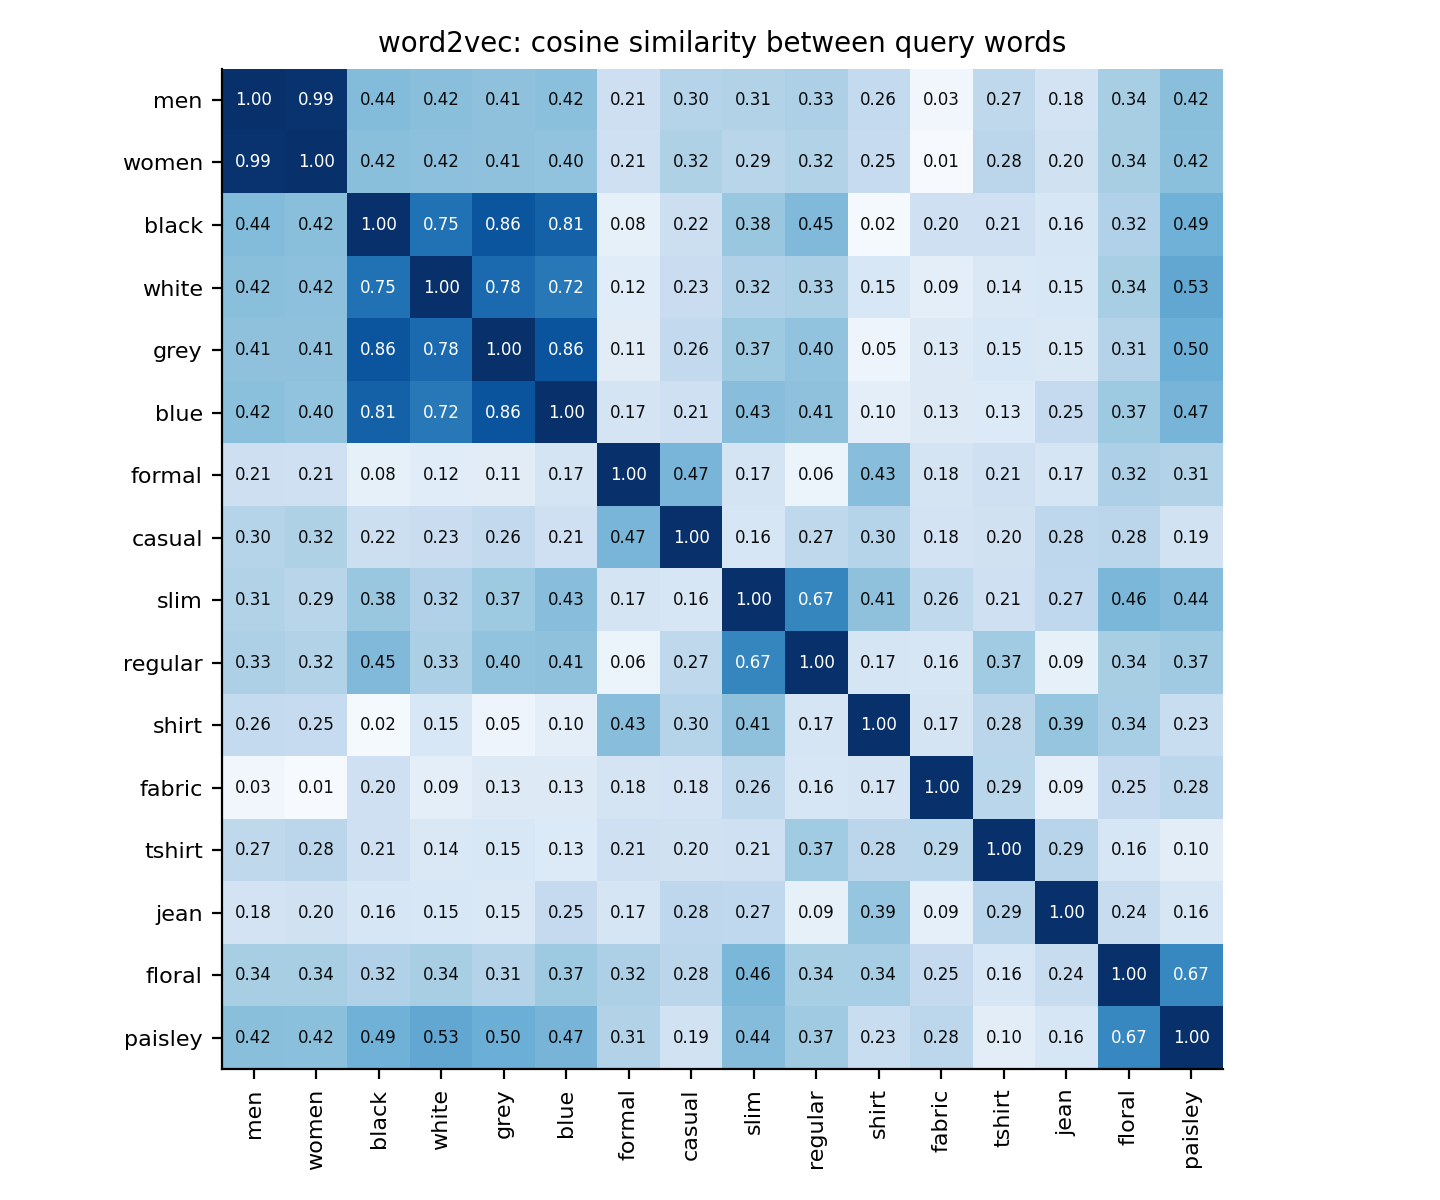
\includegraphics[width=0.58\textwidth]{figures/word2vec_similarity.png}
\caption{Cosine similarity between the word2vec vectors of some query words.}
\label{fig:w2v}
\end{figure}

\textbf{Pros:} it knows which words are related (\texttt{floral} and \texttt{paisley}, \texttt{zip} and
\texttt{closur}), so with an OR search it could find products that do not contain the exact query word; and each product
is a single dense vector. \textbf{Cons:} the average loses the word order and how important each word is (a decisive rare
word like \texttt{formal} weighs the same as \texttt{fit}); opposite attributes look alike; and rare words get poor
vectors.

%=====================================================================================================
\section{Comparison of the four rankings}
\label{sec:compare}

\begin{table}[H]
\centering\footnotesize
\setlength{\tabcolsep}{3.6pt}
\caption{Mean over the test queries Q1--Q5 (all the AND matches are labelled). Our score is the best in every column.}
\label{tab:test}
\begin{tabular}{@{}l cccc cccc cccc c@{}}
\toprule
 & \multicolumn{4}{c}{$K = 5$} & \multicolumn{4}{c}{$K = 10$} & \multicolumn{4}{c}{$K = 20$} & \\
\cmidrule(lr){2-5}\cmidrule(lr){6-9}\cmidrule(lr){10-13}
method & P & R & MAP & NDCG & P & R & MAP & NDCG & P & R & MAP & NDCG & MRR\\
\midrule
TF-IDF + cosine & .480 & .200 & .670 & .491 & .580 & .494 & .628 & .617 & .390 & .679 & .608 & .631 & .680\\
BM25 & .560 & .282 & .847 & .626 & .460 & .446 & .793 & .605 & .440 & .732 & .672 & .730 & .900\\
Our score & \best{.920} & \best{.463} & \best{.940} & \best{.923} & \best{.740} & \best{.690} & \best{.915} &
\best{.890} & \best{.480} & \best{.773} & \best{.895} & \best{.859} & \best{1.00}\\
word2vec + cosine & .640 & .282 & .666 & .597 & .580 & .465 & .698 & .628 & .450 & .710 & .653 & .674 & .640\\
\bottomrule
\end{tabular}
\end{table}

\begin{table}[H]
\centering\footnotesize
\setlength{\tabcolsep}{3.6pt}
\caption{Mean over the validation queries V1--V2 (20 labelled products per query).}
\label{tab:val}
\begin{tabular}{@{}l cccc cccc cccc c@{}}
\toprule
 & \multicolumn{4}{c}{$K = 5$} & \multicolumn{4}{c}{$K = 10$} & \multicolumn{4}{c}{$K = 20$} & \\
\cmidrule(lr){2-5}\cmidrule(lr){6-9}\cmidrule(lr){10-13}
method & P & R & MAP & NDCG & P & R & MAP & NDCG & P & R & MAP & NDCG & MRR\\
\midrule
TF-IDF + cosine & .900 & .392 & 1.00 & .934 & .800 & .685 & .974 & .858 & .475 & .800 & .951 & .852 & 1.00\\
BM25 & 1.00 & .442 & 1.00 & 1.00 & .800 & .685 & .988 & .861 & .475 & .800 & .973 & .858 & 1.00\\
Our score & 1.00 & .442 & 1.00 & 1.00 & .750 & .646 & .983 & .828 & .475 & .800 & .963 & .855 & 1.00\\
word2vec + cosine & .900 & .392 & .944 & .915 & .750 & .646 & .937 & .814 & .475 & .800 & .905 & .837 & 1.00\\
\bottomrule
\end{tabular}
\end{table}

\begin{figure}[H]
\centering
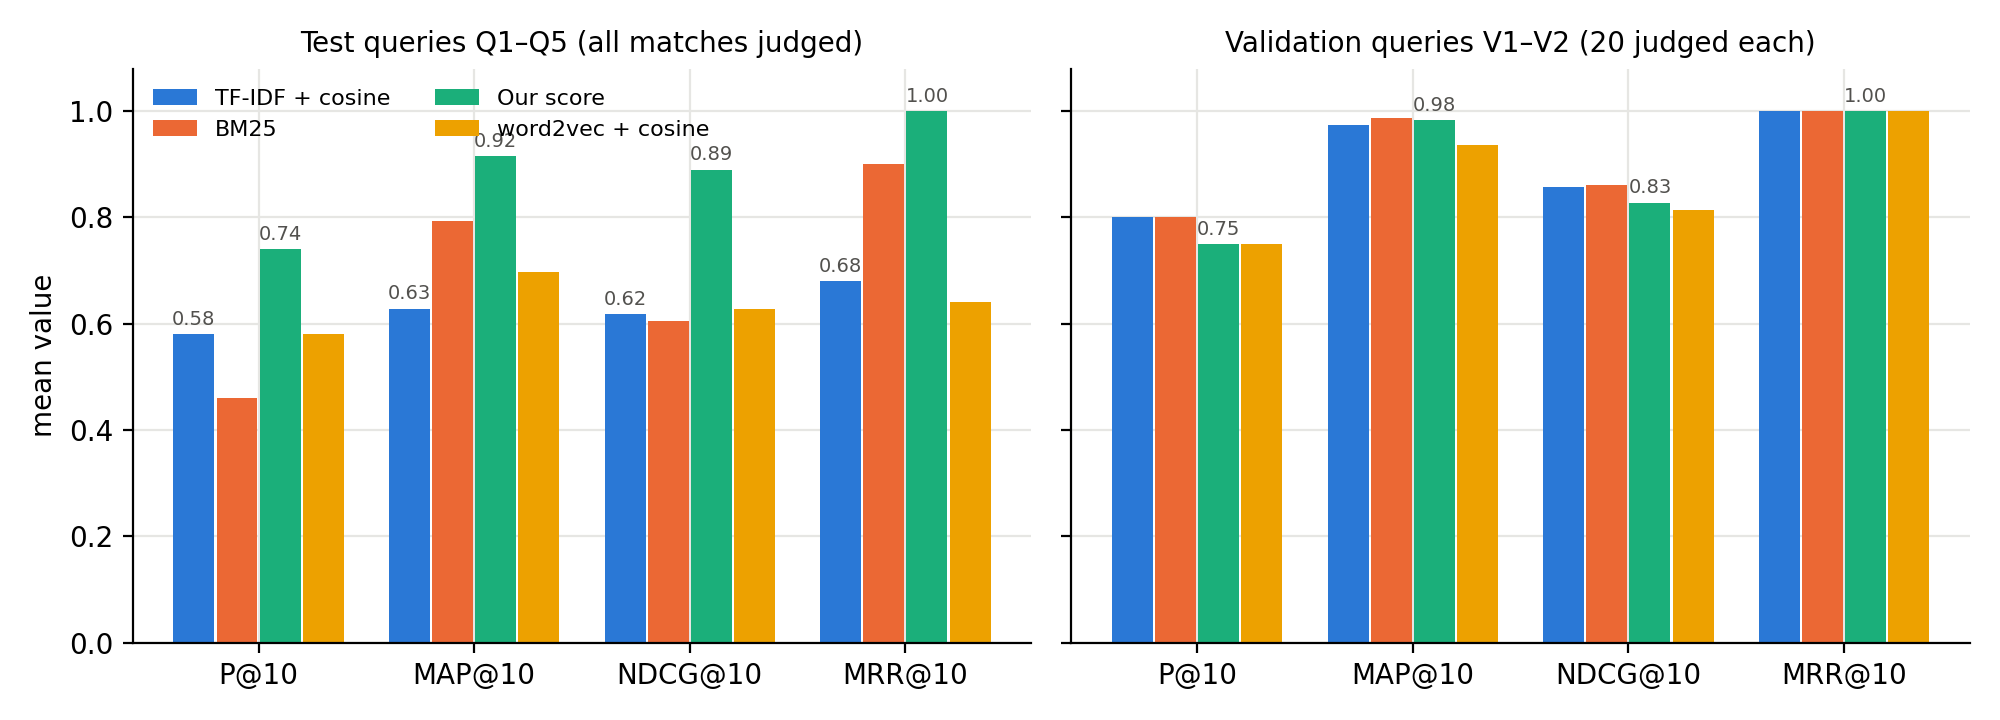
\includegraphics[width=\textwidth]{figures/metrics_by_method.png}
\caption{Main metrics at $K = 10$ for the four methods, on the test queries and on the validation queries.}
\label{fig:metrics}
\end{figure}

\begin{figure}[H]
\centering
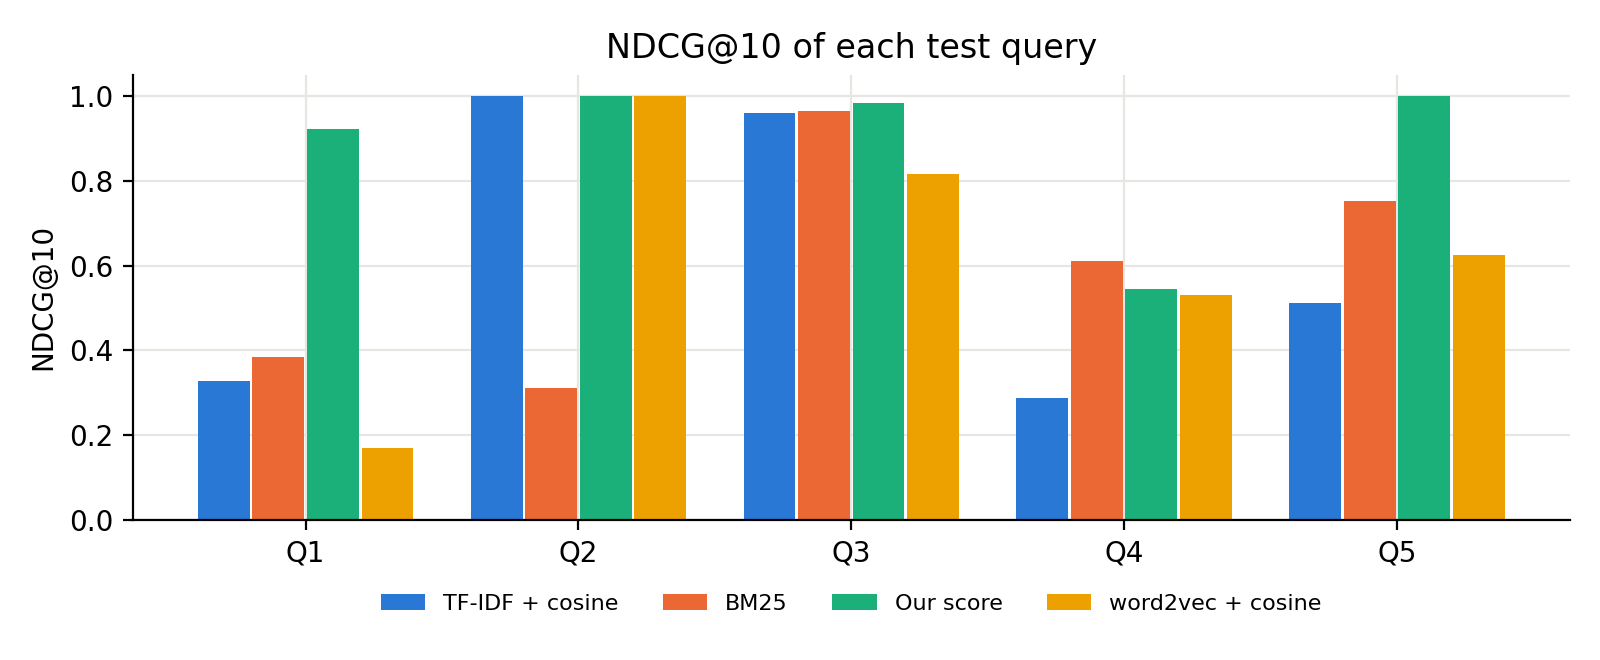
\includegraphics[width=0.8\textwidth]{figures/ndcg_per_query.png}
\caption{NDCG@10 of each method on each test query.}
\label{fig:perquery}
\end{figure}

\textbf{Test queries.} Our score is the best at every cut-off (NDCG@10 of 0.89, against 0.61--0.63 for the other
methods), and its first result is always relevant (MRR 1.00).

\textbf{Validation queries.} They are easy (all the methods have MRR 1) and they do not separate the methods much. Our
score is tied with BM25 at $K = 5$, but it is lower at $K = 10$ (NDCG@10 0.83 against 0.86). This is because the quality
factor moves a relevant product of V1 that is out of stock out of the top~10. For a shop we think this is the right
behaviour, but the metrics count it as an error.

\textbf{Per query} (Figure~\ref{fig:perquery}):
\begin{itemize}
\item \textbf{Q1} (formal or casual): only our score separates them (0.92), thanks to the title.
\item \textbf{Q2} (shirt or fabric): TF-IDF, our score and word2vec are perfect, and BM25 fails (0.31).
\item \textbf{Q3}: all the methods do well (0.96--0.98) except word2vec (0.82), which puts the men's track pants first.
\item \textbf{Q4}: the hardest query (0.29--0.61). The pre-processing removes ``3'' and ``of'', so the query becomes
\texttt{women pure cotton tshirt pack}, and no method can tell a pack of 3 from a pack of 5. This is a limit of the
pre-processing, not of the ranking.
\item \textbf{Q5}: our score is perfect (1.00), because the title factor and the field weights move the women's shoes down.
\end{itemize}

\textbf{How different are the rankings?} Two methods share between 12.8 and 15.8 of the 20 products of their top~20
(Figure~\ref{fig:overlap}). So they mostly agree on \emph{which} products are good, and they disagree on the
\emph{order}. TF-IDF and BM25 are the most similar pair (15.8), and our score is the most different from the others
(12.8--13.4). The diagonal is 18.2 and not 20 because Q3 only has 11 matches.

\begin{figure}[H]
\centering
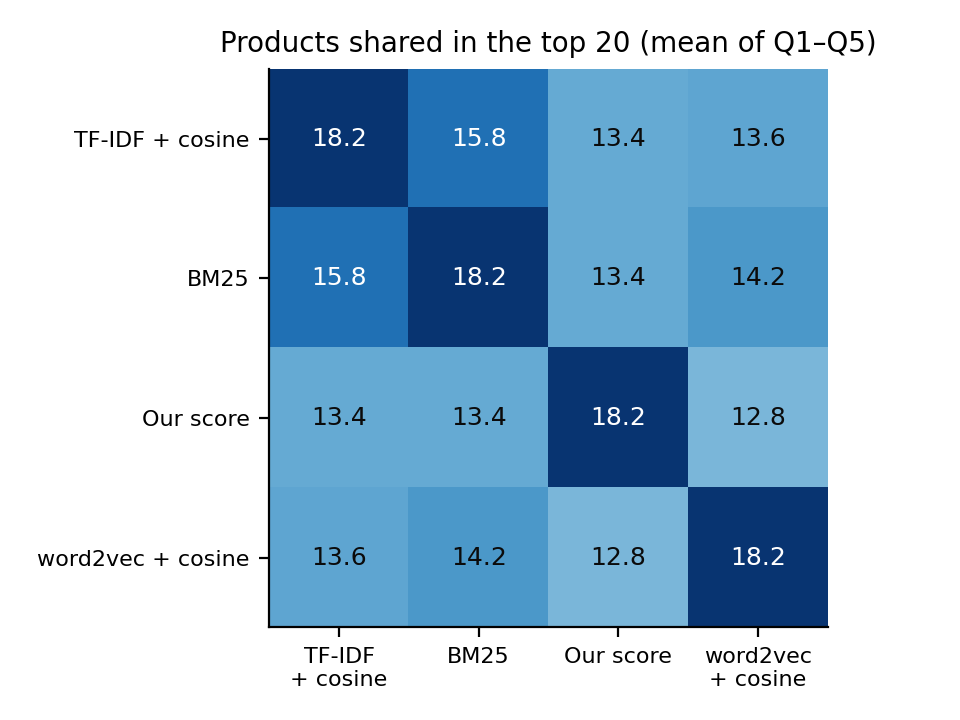
\includegraphics[width=0.48\textwidth]{figures/top20_overlap.png}
\caption{Average number of products that the top~20 of two methods have in common (Q1--Q5).}
\label{fig:overlap}
\end{figure}

%=====================================================================================================
\section{A better representation than word2vec (point 3)}

Our word2vec ranking has two weak points: (1) all the words weigh the same in the average, and (2) a word always has
the same vector, whatever its context, so \texttt{men} and \texttt{women} end up almost the same.

\begin{table}[H]
\centering\small
\caption{Ways to represent a whole text, compared with the average of the word2vec vectors.}
\label{tab:repr}
\begin{tabularx}{\textwidth}{@{}>{\raggedright}p{2.8cm}YY@{}}
\toprule
representation & pros & cons\\
\midrule
\textbf{Weighted average} of word2vec (TF-IDF or SIF weights) & rare and decisive words (\texttt{formal},
\texttt{zip}) weigh more; same model, almost no extra cost & still a bag of words; opposite attributes still look
alike\\
\addlinespace
\textbf{Doc2Vec} (PV-DM, PV-DBOW) & it learns one vector for each product, so nothing is averaged; PV-DM uses the word
order; cheap & for a new query it needs an inference step (a few training steps, which give a slightly different
vector each time); trained only on our 28,080 products, so it keeps the confusions of co-occurrence\\
\addlinespace
\textbf{Sentence embeddings} (Sentence-BERT) & it reads each word in its context, so ``men's running shoes'' and
``women's running shoes'' get different vectors; it is pre-trained on a lot of data (synonyms, paraphrases), so it does
not need our training; it can be fine-tuned with (query, product) pairs & slower (a neural network for every product and
query); a limit on the input length; harder to explain; it may still mix colours if it is not fine-tuned\\
\addlinespace
\textbf{Cross-encoder} re-ranking & it reads the query and the product together, so it can check every condition of the
query; the most accurate & too slow for all the products, so only to re-rank the top~20--50\\
\bottomrule
\end{tabularx}
\end{table}

\textbf{Our choice} would be a hybrid system. First we keep the AND search and our lexical score to get the candidates
(this way the exact attributes of the query are in the products). Then we re-rank the top~50 with sentence embeddings
(or with a cross-encoder if it is fast enough), which add the meaning. Doc2Vec would be better than the average, but
since it would only be trained on our corpus, it would still confuse attributes that appear in the same contexts. And
some conditions (the gender, the pack size of Q4) are easier to handle as structured fields extracted from the text
than with any vector.

%=====================================================================================================
\section{Assumptions and limitations}
\begin{itemize}
\item The queries are conjunctive: the ranking only changes the order of the AND matches, never which products are
returned.
\item The labels are binary and follow the criteria of Section~1. Stock, rating and discount are not part of relevance.
\item We only have five test queries and two validation queries, so the differences are indicative, and a single query
can change a mean a lot.
\item We set the weights of our score before testing it. The BM25 grid only shows how sensitive BM25 is (we kept the
standard values).
\item The pre-processing removes numbers, so pack sizes (Q4) cannot be matched. Keeping the number that follows words like
``pack'' would fix it.
\end{itemize}

\section*{Use of AI tools}
We used an AI assistant (Claude) during this part. It helped us to refactor and debug parts of the code and to make the
figures. We used it to brainstorm ideas but we decided the methods and the criteria, labelled the products and
checked the results ourselves.

\newpage
\appendix
\section{word2vec + cosine: top-20 results of the test queries}
\label{app:w2v}
The column ``rel.'' is our relevance label (\checkmark{} = relevant). The same lists are in the file
\texttt{results/word2vec\_top20.csv}, and the top~20 of all four methods are in the file
\texttt{results/top20\_all\_methods.csv}.

\begin{table}[H]\centering\scriptsize
\caption{word2vec + cosine: top 20 of Q1 (\emph{men white formal shirt slim fit}). 7 of the 20 results are relevant.}
\begin{tabular}{@{}rlccl@{}}\toprule
rank & pid & rel. & score & title\\\midrule
1 & \texttt{SHTF6VCHUQ8HKQPE} & -- & 0.903 & Men Slim Fit Solid Casual Shirt\\
2 & \texttt{SHTFEBYMF9RTZYKG} & -- & 0.903 & Men Slim Fit Solid Spread Collar Casual Shirt\\
3 & \texttt{SHTFEBYMGU47WWZG} & -- & 0.903 & Men Slim Fit Solid Spread Collar Casual Shirt\\
4 & \texttt{SHTFEBYMHVXRHZCZ} & -- & 0.903 & Men Slim Fit Solid Spread Collar Casual Shirt\\
5 & \texttt{SHTFDYRQRYGTW4PX} & \checkmark & 0.867 & Men Slim Fit Printed Button Down Collar Formal Shirt\\
6 & \texttt{SHTFDYTZGHNN2JQ9} & -- & 0.861 & Men Slim Fit Polka Print Button Down Collar Casual Shirt\\
7 & \texttt{SHTFW52ZURHFKNTZ} & \checkmark & 0.861 & Men Slim Fit Printed Button Down Collar Formal Shirt\\
8 & \texttt{SHTFDYMU7MCMFCT9} & -- & 0.857 & Men Slim Fit Geometric Print Button Down Collar Casual Shirt\\
9 & \texttt{SHTFW52ZMFEJNWYY} & -- & 0.852 & Men Slim Fit Printed Club Collar Casual Shirt\\
10 & \texttt{TROFYFX6XK4HYZFN} & -- & 0.842 & Slim Fit Men White Cotton Blend Trousers\\
11 & \texttt{SHTFW52ZMBHJZPYP} & \checkmark & 0.832 & Men Slim Fit Printed Spread Collar Formal Shirt\\
12 & \texttt{SHTFCCRGK52CM7YR} & -- & 0.805 & Men Slim Fit Checkered Spread Collar Formal Shirt\\
13 & \texttt{SHTF98P8MTY7ZXAZ} & \checkmark & 0.794 & Men Slim Fit Solid Spread Collar Formal Shirt\\
14 & \texttt{SHTF8XMFDHS4WFFT} & -- & 0.791 & Men Regular Fit Checkered Spread Collar Formal Shirt\\
15 & \texttt{SHTFZTRSN4HXHMHH} & -- & 0.790 & Men Regular Fit Solid Spread Collar Formal Shirt\\
16 & \texttt{SHTFZTRSPEK26PYJ} & -- & 0.790 & Men Regular Fit Solid Spread Collar Formal Shirt\\
17 & \texttt{SHTFFVYPMWHZ3SFQ} & -- & 0.781 & Men Slim Fit Checkered Spread Collar Formal Shirt\\
18 & \texttt{SHTFU73NHNAFBCCZ} & \checkmark & 0.776 & Men Slim Fit Solid Spread Collar Formal Shirt\\
19 & \texttt{SHTFU73NP63MDZZP} & \checkmark & 0.776 & Men Slim Fit Solid Spread Collar Formal Shirt\\
20 & \texttt{SHTFU73NTX6N3R63} & \checkmark & 0.776 & Men Slim Fit Solid Spread Collar Formal Shirt\\
\bottomrule\end{tabular}\end{table}
\begin{table}[H]\centering\scriptsize
\caption{word2vec + cosine: top 20 of Q2 (\emph{women floral print shirt}). 16 of the 20 results are relevant.}
\begin{tabular}{@{}rlccl@{}}\toprule
rank & pid & rel. & score & title\\\midrule
1 & \texttt{SHTFHQTAZZVYHZGY} & \checkmark & 0.894 & Women Slim Fit Floral Print Casual Shirt\\
2 & \texttt{SHTFJZC45ZFYGSYH} & \checkmark & 0.890 & Women Slim Fit Floral Print Casual Shirt\\
3 & \texttt{SHTFSYG8TVBV8SUK} & \checkmark & 0.862 & Women Slim Fit Floral Print Casual Shirt\\
4 & \texttt{SHTFTGV4HRGGY4Z7} & \checkmark & 0.857 & Women Regular Fit Floral Print Button Down Collar Casual Shirt\\
5 & \texttt{SHTFTGV4ATUQYVWY} & \checkmark & 0.855 & Women Regular Fit Floral Print Button Down Collar Casual Shirt\\
6 & \texttt{SHTFS6YAFFX5XFFH} & \checkmark & 0.855 & Women Slim Fit Floral Print Casual Shirt\\
7 & \texttt{SHTFTGV4UGTG5HZH} & \checkmark & 0.854 & Women Regular Fit Floral Print Button Down Collar Casual Shirt\\
8 & \texttt{SHTFWD49GF2EA3UN} & \checkmark & 0.844 & Women Slim Fit Printed Slim Collar Casual Shirt\\
9 & \texttt{SHTFMRH8WRCFQMYF} & \checkmark & 0.835 & Women Slim Fit Floral Print Spread Collar Casual Shirt\\
10 & \texttt{SHTF4FWJ6UQAHRQM} & \checkmark & 0.834 & Women Regular Fit Floral Print Casual Shirt\\
11 & \texttt{SHTF45DYRFA4M4AZ} & \checkmark & 0.833 & Women Regular Fit Floral Print Spread Collar Casual Shirt\\
12 & \texttt{FABFZU8HREHCNJR5} & -- & 0.812 & Rayon Printed, Floral Print Shirt Fabric (Unstitched)\\
13 & \texttt{SHTFDYMYV7AUKE9R} & \checkmark & 0.807 & Women Slim Fit Floral Print Button Down Collar Casual Shirt\\
14 & \texttt{SHTF47JNQFEFRQHG} & \checkmark & 0.806 & Women Regular Fit Printed Button Down Collar Casual Shirt\\
15 & \texttt{SHTF47JNAVU4UMVP} & \checkmark & 0.806 & Women Regular Fit Printed Button Down Collar Casual Shirt\\
16 & \texttt{FABFZU92QEBHMCZB} & -- & 0.792 & Rayon Floral Print, Self Design Shirt Fabric (Unstitched)\\
17 & \texttt{SHTFEQJA48XC5WX4} & \checkmark & 0.788 & Women Slim Fit Printed Club Collar Casual Shirt\\
18 & \texttt{SHTFV5GYNPY6EMZS} & \checkmark & 0.782 & Women Slim Fit Floral Print Cut Away Collar Casual Shirt\\
19 & \texttt{FABFZU9YG9FZGWCY} & -- & 0.780 & Rayon Floral Print Shirt Fabric (Unstitched)\\
20 & \texttt{FABFZFR2ETCKRZJE} & -- & 0.776 & Cotton Floral Print Shirt Fabric (Unstitched)\\
\bottomrule\end{tabular}\end{table}
\begin{table}[H]\centering\scriptsize
\caption{word2vec + cosine: Q3 (\emph{women black track pants with zip pockets}): the query has only 11 AND matches, so all of them are listed. 8 of the 11 are relevant.}
\begin{tabular}{@{}rlccl@{}}\toprule
rank & pid & rel. & score & title\\\midrule
1 & \texttt{TKPFK5KGEUPYCAUH} & -- & 0.843 & Solid Men Black Track Pants\\
2 & \texttt{TKPFDT6GHGEYDTAS} & \checkmark & 0.820 & Solid Women Black Track Pants\\
3 & \texttt{TKPFKFZFXZT5XQYZ} & \checkmark & 0.798 & Solid Women Black, Grey Track Pants\\
4 & \texttt{TKPFUBDB8WGRDDYJ} & \checkmark & 0.796 & Solid Women Black Track Pants\\
5 & \texttt{TKPFWGMH448EGQTF} & \checkmark & 0.795 & Solid Women Black Track Pants\\
6 & \texttt{TKPFKFK4ESGQ95CK} & \checkmark & 0.786 & Solid Women Black Track Pants\\
7 & \texttt{TKPFRAHGFDFBHZ3J} & \checkmark & 0.777 & Solid Women Black Track Pants\\
8 & \texttt{TKSF5WHGCR4JBXYZ} & -- & 0.772 & Regular Fit Women Black Cotton Lycra Blend Trousers\\
9 & \texttt{TKPFDGYPBYPAZNXH} & \checkmark & 0.761 & Self Design Women Black Track Pants\\
10 & \texttt{TKPFN5S8QKWKFHCM} & \checkmark & 0.736 & Solid Women Black Track Pants\\
11 & \texttt{TKPFUY98MWHVV2W5} & -- & 0.712 & Printed Women Black Track Pants\\
\bottomrule\end{tabular}\end{table}
\begin{table}[H]\centering\scriptsize
\caption{word2vec + cosine: top 20 of Q4 (\emph{women pure cotton t-shirt pack of 3}). 9 of the 20 results are relevant.}
\begin{tabular}{@{}rlccl@{}}\toprule
rank & pid & rel. & score & title\\\midrule
1 & \texttt{TSHFWAWKMVHVWC5P} & -- & 0.834 & Solid Women Round Neck Multicolor T-Shirt (Pack of 5)\\
2 & \texttt{TSHFWBWEXX3N9FHZ} & \checkmark & 0.832 & Solid Women Round Neck Blue, Maroon T-Shirt (Pack of 3)\\
3 & \texttt{TSHFWAWKHFZDGSVX} & -- & 0.832 & Solid Women Round Neck Multicolor T-Shirt (Pack of 5)\\
4 & \texttt{TSHFWBWEV3J285KG} & \checkmark & 0.832 & Solid Women Round Neck Blue T-Shirt (Pack of 3)\\
5 & \texttt{TSHFWBWERWBHYYJG} & \checkmark & 0.831 & Solid Women Round Neck Grey T-Shirt (Pack of 3)\\
6 & \texttt{TSHFWBWECMBZ9D8A} & \checkmark & 0.831 & Solid Women Round Neck Black T-Shirt (Pack of 3)\\
7 & \texttt{TSHFWAWKK2GNAQJA} & -- & 0.831 & Solid Women Round Neck Maroon T-Shirt (Pack of 5)\\
8 & \texttt{TSHFWBWEGZEDCABK} & \checkmark & 0.831 & Solid Women Round Neck Maroon T-Shirt (Pack of 3)\\
9 & \texttt{TSHFWAWKKGYZSNHU} & -- & 0.830 & Solid Women Round Neck Grey T-Shirt (Pack of 5)\\
10 & \texttt{TSHFVYHBZYHZGEGJ} & \checkmark & 0.828 & Solid Women Round Neck Multicolor T-Shirt (Pack of 3)\\
11 & \texttt{TSHFVYHBU7AKH4E8} & \checkmark & 0.825 & Solid Women Round Neck Multicolor T-Shirt (Pack of 3)\\
12 & \texttt{TSHFXS3FD6N7FDYK} & -- & 0.823 & Solid Women Round Neck Black, White T-Shirt (Pack of 2)\\
13 & \texttt{TSHFVYHB7YTVJ77M} & \checkmark & 0.823 & Solid Women Round Neck Multicolor T-Shirt (Pack of 3)\\
14 & \texttt{TSHFHPJYUXBJVSQN} & -- & 0.817 & Self Design, Solid Women Round Neck Black T-Shirt (Pack of 2)\\
15 & \texttt{TSHFXS3FFH8KWZF4} & -- & 0.817 & Solid Women Round Neck White, Blue T-Shirt (Pack of 2)\\
16 & \texttt{TSHFYRYBKCSQNGGS} & -- & 0.816 & Solid Women Round Neck White T-Shirt (Pack of 4)\\
17 & \texttt{TSHFYRYBJFBSGCHS} & \checkmark & 0.814 & Solid Women Round Neck Black, Blue, White T-Shirt (Pack of 3)\\
18 & \texttt{TSHFGPZ2HVZDWUHQ} & -- & 0.813 & Solid Women Round Neck Black, White T-Shirt (Pack of 2)\\
19 & \texttt{TSHFYRYBHWBHF4WU} & -- & 0.812 & Solid Women Round Neck Blue T-Shirt (Pack of 4)\\
20 & \texttt{TSHFYRYBGYSGFHU8} & -- & 0.812 & Solid Women Round Neck Black, White T-Shirt (Pack of 4)\\
\bottomrule\end{tabular}\end{table}
\begin{table}[H]\centering\scriptsize
\caption{word2vec + cosine: top 20 of Q5 (\emph{black running shoes for men}). 5 of the 20 results are relevant.}
\begin{tabular}{@{}rlccl@{}}\toprule
rank & pid & rel. & score & title\\\midrule
1 & \texttt{SHOEKNRJ34UCMAPA} & \checkmark & 0.904 & SPRINT Running Shoes For Men (Black, Grey)\\
2 & \texttt{SHOFN3EJHXHGSGUC} & \checkmark & 0.882 & RS-7250 Running Shoes For Men (Black)\\
3 & \texttt{SHOFTZFQP8W9G86F} & -- & 0.796 & Running Shoes For Women (Black)\\
4 & \texttt{SHOFTZFPNCU4VWHK} & \checkmark & 0.796 & Running Shoes For Men (Black)\\
5 & \texttt{SHOFKH9ZNNNWCHGC} & -- & 0.762 & Running Shoes For Men (Blue)\\
6 & \texttt{SHOFZP2FHH8Z6ZHC} & -- & 0.755 & Running Shoes For Women (Black)\\
7 & \texttt{SHOFRCTVKE4P38CH} & -- & 0.753 & Target Full Spike Cricket Shoes For Men (White, Black)\\
8 & \texttt{SHOFVXG5XR59AFTH} & -- & 0.743 & Lace Up For Men (Black)\\
9 & \texttt{SHOFVJX2TP8FRR7P} & -- & 0.740 & Lace Up For Men (Black)\\
10 & \texttt{SHOFVHY8MAYUPTZF} & -- & 0.735 & Loafers For Men (Black)\\
11 & \texttt{SHOFUH52V5AVNHMN} & -- & 0.721 & Loafers For Men (Black)\\
12 & \texttt{SHOFX2G6FHVNAHZN} & -- & 0.713 & Loafers For Women (Black)\\
13 & \texttt{SHOFU9EDGSMHWJS6} & -- & 0.713 & VX-7.0 Running Shoes For Women (Green, Black)\\
14 & \texttt{SHOFU9EEZG46B55M} & \checkmark & 0.712 & VX-7.0 Running Shoes For Men (Maroon, Black)\\
15 & \texttt{SHOF3A22BBDQQY8F} & \checkmark & 0.709 & Running Shoes For Men (Black, Grey)\\
16 & \texttt{SHOFN3ENUBVRD3ZX} & -- & 0.708 & RS-7050 Running Shoes For Women (Grey, Black)\\
17 & \texttt{SHOFJGUAGAVDZ8CJ} & -- & 0.704 & Slip On For Men (Black)\\
18 & \texttt{SHOEYF5UUUHKHN9X} & -- & 0.704 & Running Shoes For Women (Black)\\
19 & \texttt{SRTFGZY9PZNCD3BM} & -- & 0.703 & Printed Men Black Sports Shorts\\
20 & \texttt{SHOF34H376KMSK9Y} & -- & 0.701 & Running Shoes For Women (Black, Grey)\\
\bottomrule\end{tabular}\end{table}

\end{document}
